\clearpage
\section{Data sets and simulated samples\label{sec:samples}}

\subsection{Data sets\label{sec:datasets}}

The following datasets are used to populate the hadronic and
control samples. They correspond to the full data run of 2012 and an
integrated luminosity of $19.45 \pm 0.8\fbinv$. Only certified luminosity
sections that pass good data quality criteria are used for data taken in  
the run range 190456--208686.

\begin{table}[h]
  \caption{Datasets.}
  \label{tab:datasets}
  \centering
  \scriptsize
  \begin{tabular}{ lc }
    \hline
    \hline
    Dataset & Luminosity (fb$^{-1}$) \\
    \hline
    %/HT/Run2012A-22Jan2013-v1/AOD! & 0.87 \\     
    %/HTMHTParked/Run2012B-22Jan2013-v1/AOD! & 4.43 \\   
    %/HTMHTParked/Run2012C-22Jan2013-v1/AOD! & 6.89 \\   
    %/HTMHTParked/Run2012D-22Jan2013-v1/AOD! & 7.26 \\
    \multicolumn{1}{r}{Hadronic} & 19.45 \\ [0.5ex]
    %\verb!/HT/Run2012A-22Jan2013-v1/AOD! & n/a \\   
    %\verb!/JetHT/Run2012B-22Jan2013-v1/AOD! & n/a \\   
    %\verb!/JetHT/Run2012C-22Jan2013-v1/AOD! & n/a \\   
    %\verb!/JetHT/Run2012D-22Jan2013-v1/AOD! & n/a \\
    %\multicolumn{1}{r}{Total} & 18.33 \\ [0.5ex]
    %\verb!/SingleMu/Run2012A-22Jan2013-v1/AOD! & 0.88 \\   
    %\verb!/SingleMu/Run2012B-22Jan2013-v1/AOD! & 4.42 \\   
    %\verb!/SingleMu/Run2012C-22Jan2013-v1/AOD! & 7.12 \\   
    %\verb!/SingleMu/Run2012D-22Jan2013-v1/AOD! & 7.30 \\
    \multicolumn{1}{r}{Muon} & 19.72 \\ [0.5ex] % 19.13
%    \verb!/Photon/Run2012A-22Jan2013-v1/AOD! & 0.87 \\   
%    \verb!/SinglePhoton/Run2012B-22Jan2013-v1/AOD! & 4.42 \\   
%    \verb!/SinglePhoton/Run2012C-22Jan2013-v1/AOD! & 7.11 \\   
%    \verb!/SinglePhotonParked/Run2012D-22Jan2013-v1/AOD! & 7.23 \\
    \multicolumn{1}{r}{Photon} & 19.63 \\ [0.5ex] % 19.18
    \hline
    \hline
  \end{tabular}
\end{table}

\subsection{Simulated samples for SM backgrounds\label{sec:mc-samples}}

The SM background Monte Carlo samples for physics at 8\TeV are taken
from the \verb!Summer12! simulation production run with CMS reconstruction
software version \verb!5.3.X! with pilup scenario 10. The effective
luminosity of each MC sample is normalized to the integrated
luminosity of the corresponding dataset, as listed in
Table~\ref{tab:mc-sm}.  All MC samples are reweighted on an 
event-by-event basis such that the distribution of pile-up (PU) 
interactions matches that observed in data~\cite{pu-reweight}.

\begin{center}
  \begin{table}[h]
    \caption{MC samples for Standard Model processes.}
    \label{tab:mc-sm}
    \centering
    \tiny
    \begin{tabular}{ lrrrr }
      \hline
      Sample & HT (GeV) & Cross section (pb) & Corrected Cross section (pb) \\%& Luminosity (fb$^{-1}$) \\ %& N$_{\textrm{event}}$ 
      \hline
      \hline
      \wlnu  		& Inclusive         & 37509.0 & 34133.2  \\   %& 57661905   & 1.5    
      \wlnu  		& 150 - 200         & 253.8   & 234.53   \\   %& 21414209   & 84.4   
      \wlnu  		& 200 - 250         & 116.5   & 103.94   \\   %& 9895771    & 84.9   
      \wlnu  		& 250 - 300         & 57.6    & 51.34    \\   %& 4924990    & 85.5   
      \wlnu  		& 300 - 400         & 48.4    & 42.41    \\   %& 5141023    & 106.2  
      \wlnu  		& 400 - $\infty$    & 30.8    & 26.36    \\   %& 4923847    & 159.9
      \znunu 		& 50 - 100          & 452.8   & 405.21   \\   %& 23743998   & 52.4   
      \znunu 		& 100 - 200         & 190.4   & 173.76   \\   %& 9876059    & 51.9   
      \znunu 		& 200 - 400         & 45.1    & 42.41    \\   %& 9649619    & 214.0  
      \znunu 		& 400 - $\infty$    & 6.26    & 5.81     \\   %& 5079710    & 811.5
      \ttbar          & Inclusive         & 234.0   & 271.44   \\   %& 115.8   \\   %& 27094723 
      \dyllFifty      & Inclusive         & 3503.7  & 3258.45  \\   %& 8.6     \\   %& 30171503 
      \dyllTen        & Inclusive         & 13124.1 & 12205.4  \\   %& 0.5     \\   %& 7116223  \\
      \dyll           & 200 - 400         & 24.3    & 22.24    \\   %& 283.7   \\   %& 6892777  
      \dyll           & 400 - $\infty$    & 3.36    & 3.11     \\   %& 802.3   \\   %& 2695789  
      \gj             & 200 - 400         & 1140.8  & 1060.9   \\   %& 50.7    \\   %& 57891147  
      \gj             & 400 - $\infty$    & 124.7   & 115.97   \\   %& 75.9    \\   %& 9459562   
      WW              & Inclusive         & 57.1    & 57.1     \\   %& 173.2   \\   %& 9888431  
      WZ              & Inclusive         & 12.6    & 12.6     \\   %& 781.1   \\   %& 9841248  
      ZZ              & Inclusive         & 8.26    & 8.26     \\   %& 1180.6  \\   %& 9751908  
      \ttc            & Inclusive         & 56.4    & 56.4     \\   %& 65.8    \\   %& 3710227  
      \tbtc           & Inclusive         & 30.7    & 30.7     \\   %&  63.0    \\   %& 1935072  
      \tsc            & Inclusive         & 3.79    & 3.79     \\   %& 64.4    \\   %& 243961   
      \tbsc           & Inclusive         & 1.76    & 1.76     \\   %& 79.5    \\   %& 139974   
      \ttwc           & Inclusive         & 11.1    & 11.1     \\   %& 44.8    \\   %& 497658   
      \tbtwc          & Inclusive         & 11.1    & 11.1     \\   %& 44.5    \\   %& 493460   
      %\verb!/QCD_Pt-50to80_TuneZ2star_8TeV_pythia6/Summer12_DR53X-PU_S10_START53_V7A-v2!                        & 5950860  & 8148778 & 8148778 (LO) & 0.001   \\     
      %\verb!/QCD_Pt-80to120_TuneZ2star_8TeV_pythia6/Summer12_DR53X-PU_S10_START53_V7A-v3!                       & 5962864  & 1033680 & 1033680 (LO) & 0.006   \\     
      %\verb!/QCD_Pt-120to170_TuneZ2star_8TeV_pythia6/Summer12_DR53X-PU_S10_START53_V7A-v3!                      & 5985732  & 156293  & 156293  (LO) & 0.038   \\     
      %\verb!/QCD_Pt-170to300_TuneZ2star_8TeV_pythia6/Summer12_DR53X-PU_S10_START53_V7A-v1(v2)!                  & 20155180 & 34138   & 34138   (LO) & 0.590   \\     
      %\verb!/QCD_Pt-300to470_TuneZ2star_8TeV_pythia6/Summer12_DR53X-PU_S10_START53_V7A-v1(v2,v3)!               & 23588100 & 1759.5  & 1759.5  (LO) & 13.4    \\    
      %\verb!/QCD_Pt-470to600_TuneZ2star_8TeV_pythia6/Summer12_DR53X-PU_S10_START53_V7A-v2!                      & 3978848  & 113.9   & 113.9   (LO) & 34.9    \\    
      %\verb!/QCD_Pt-600to800_TuneZ2star_8TeV_pythia6/Summer12_DR53X-PU_S10_START53_V7A-v2!                      & 3964864  & 27.0    & 27.0    (LO) & 146.8   \\   
      %\verb!/QCD_Pt-800to1000_TuneZ2star_8TeV_pythia6/Summer12_DR53X-PU_S10_START53_V7A-v2!                     & 3854563  & 3.55    & 3.55    (LO) & 1085.8  \\  
      %\verb!/QCD_Pt-1000to1400_TuneZ2star_8TeV_pythia6/Summer12_DR53X-PU_S10_START53_V7A-v1!                    & 1964088  & 0.738   & 0.738   (LO) & 2661.4  \\  
      %\verb!/QCD_Pt-1400to1800_TuneZ2star_8TeV_pythia6/Summer12_DR53X-PU_S10_START53_V7A-v1!                    & 1988062  & 0.0335  & 0.0335  (LO) & 59345.1 \\ 
      %\verb!/QCD_Pt-1800_TuneZ2star_8TeV_pythia6/Summer12_DR53X-PU_S10_START53_V7A-v1!                          & 977586   & 0.00183 & 0.00183 (LO) & 534200  \\
      \hline
    \end{tabular}
  \end{table}
\end{center}
%\end{landscape}
%
%\begin{landscape}
%  \begin{center}
%    \begin{table}[h]
%      \caption{MC samples for simplified models.}
%      \label{tab:mc-signal}
%      \centering
%      \tiny
%      \begin{tabular}{ lll }
%        \hline
%        Model & Sample & Description \\
%        \hline
%        \hline
%        \verb!T2cc! & \verb!/SMS-MadGraph_2J_T2cc_NoFilter_mStop-100to250_mLSP-20to230_8TeV-Pythia6Zstar/Summer12-START52_V9_FSIM-v1/AODSIM! & Original scan \\   
%        \verb!T2cc! & \verb!/SMS-T2cc_NoFilter_mStop-175to250_mLSP-95to240_8TeV-Pythia6Z/Summer12-START52_V9_FSIM-v1/AODSIM! & Original scan \\   
%        \verb!T2cc! & \verb!/SMS-T2cc_2J_mStop-250to350_mLSP-195to340_TuneZ2star_8TeV-madgraph-tauola/Summer12-START53_V19_FSIM-v2/AODSIM! & Scan extension \\   
%        \verb!T2cc! & \verb!/SMS-8TeV_Pythia6Z_T2cc_3jets_mStop-200_mLSP-120/Summer12-START52_V9_FSIM-v1/AODSIM! & 3-parton sample \\   
%        \verb!T2cc! & \verb!/SMS-8TeV_Pythia6Z_T2cc_3jets_mStop-200_mLSP-190/Summer12-START52_V9_FSIM-v1/AODSIM! & 3-parton sample \\   
%        \hline
%        \hline
%      \end{tabular}
%    \end{table}
%  \end{center}
%\end{landscape}
%
%%\subsection{Weighting MC samples according to the pile-up distribution
%%  in data}
%%
%%All MC samples are reweighted on an event-by-event basis such that the
%%distribution of pile-up (PU) interactions matches that observed in
%%data. This is done using the recommended recipe and the PU JSON of
%%9$^{\textrm{th}}$~September 2012. Figure~\ref{fig:nvtx} shows the
%%number of reconstructed vertices in data and from simulation after
%%reweighting the MC samples using the PU JSON. Event after reweighting,
%%excellent agreement between data and MC is not expected given the
%%difficulties in correctly modelling the number of reconstructed
%%vertices in MC. However, good agreement is found between data and MC
%%for the core of the distribution.
%%
%%\begin{figure}[!h]
%%  \begin{center}
%%    \includegraphics[width=0.6\textwidth]{figures/data-mc/v1/nvtx/Stack_nVertex_Muon_all_OneMuon_-1To-2b_log}
%%    \caption{Comparison of the number of vertices reconstructed in
%%      data and MC simulation for the single muon + jet control sample,
%%      after reweighting all MC samples to match the distribution of PU
%%      interactions observed in data.\label{fig:nvtx}}
%%  \end{center}
%%\end{figure}

\subsection{Corrections to cross sections for SM samples\label{sec:k-factors}}

Every simulated event is weighted by the total number of events in the MC sample, 
the theoretical cross section, and total luminosity of the data being studied.
Theoretical calculations are available that provide next-to-next-to 
leading order (NNLO) cross sections for each inclusive SM sample~\cite{twiki-xs}. In an attempt to 
provide higher statistics in tails of distribution analyses often cut on 
(ie \partonht, \nparton, \pthat), MC samples are produced binned in these
 variables. Only the leading-order (LO) cross sections are provided~\cite{prep}, 
but in general, the \kfactors required to go from LO to NNLO cross sections
are determined using corresponding inclusive samples and applied to each binned sample. 

Studies conducted by other analyses ~\cite{RobXS} revealed that some LO cross
sections calculated for MC samples binned according to \partonht are
inaccurate to a level as large as 10\%, leading to non-physical discontinuities 
in the \partonht distribution constructed from the binned samples of a given process.
Furthermore, due to an error in production, the \wlnu \; \scalht binned samples exhibit 
\scalht-dependent biases. The following paragraphs describe a procedure to measure 
corrections to the discontinuities and biases of the \wlnu \; \partonht binned samples 
as a function of \scalht. Other analyses created similar procedures to correct 
the \zmumu \; \partonht binned samples, this analysis uses those measured corrections 
as k-factors.  

\begin{figure}[h!t]
  \begin{center}
    \subfigure[\label{fig:xsec_study_before}Parton \scalht distribution for the \wlnu inclusive sample (blue) and
    \wlnu \nparton binned sample (orange.)]{
      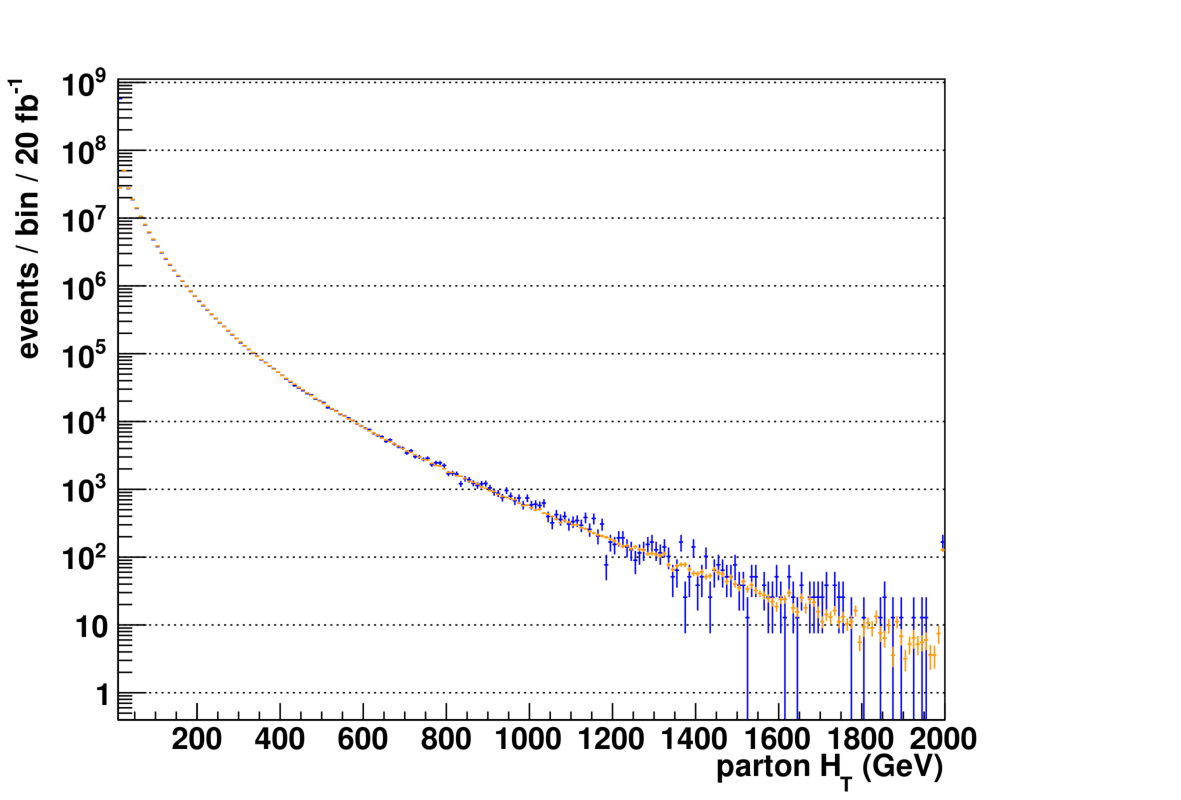
\includegraphics[width=0.6\textwidth,]{figures/samples/xs_wj_lv_mg_ht_incl_over_excl-2.pdf}
    } \\
    \subfigure[\label{fig:xsec_study_before}Fitted Parton \scalht distribution for the \wlnu \partonht sample (red) and
    \wlnu \nparton binned sample (orange.)]{
      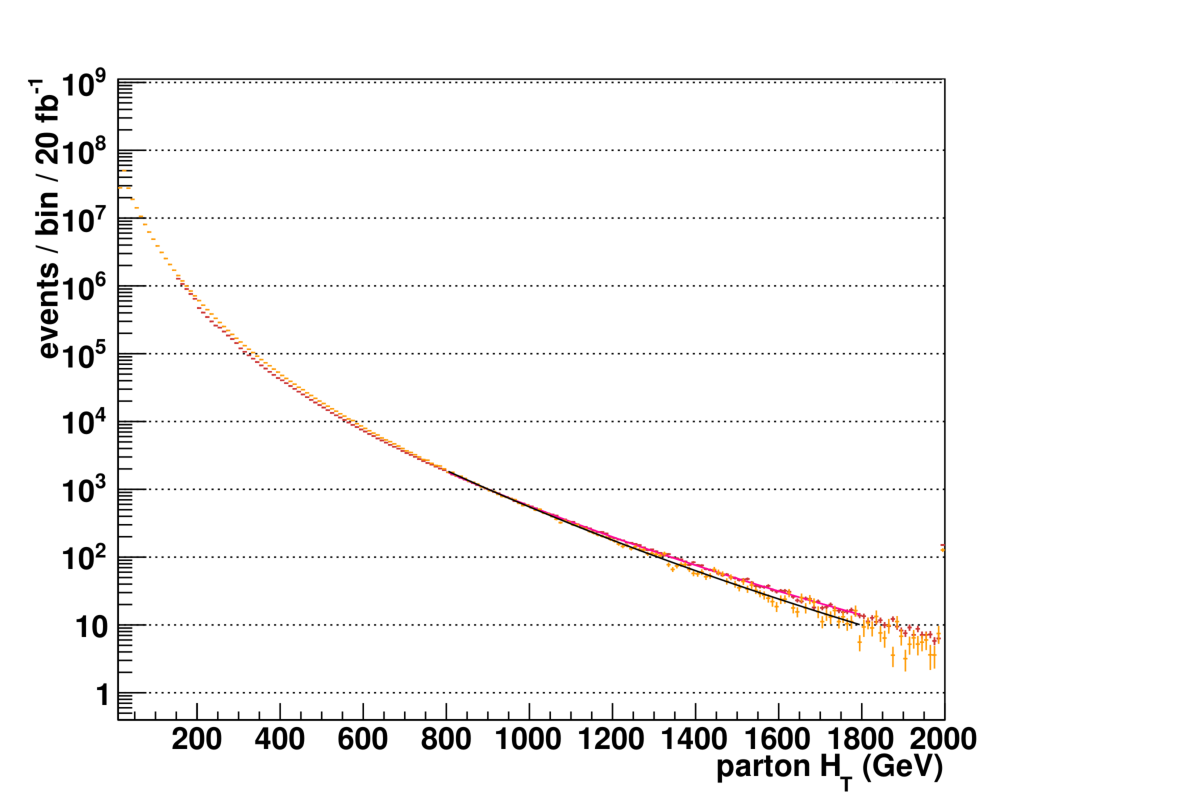
\includegraphics[width=0.6\textwidth,]{figures/samples/xs_wj_lv_mg_ht_incl_over_excl-6.pdf}
    } \\
    \subfigure[\label{fig:xsec_study_after}Event weight determined from ratio of Figure~\ref{fig:xsec_study} (b)]{
      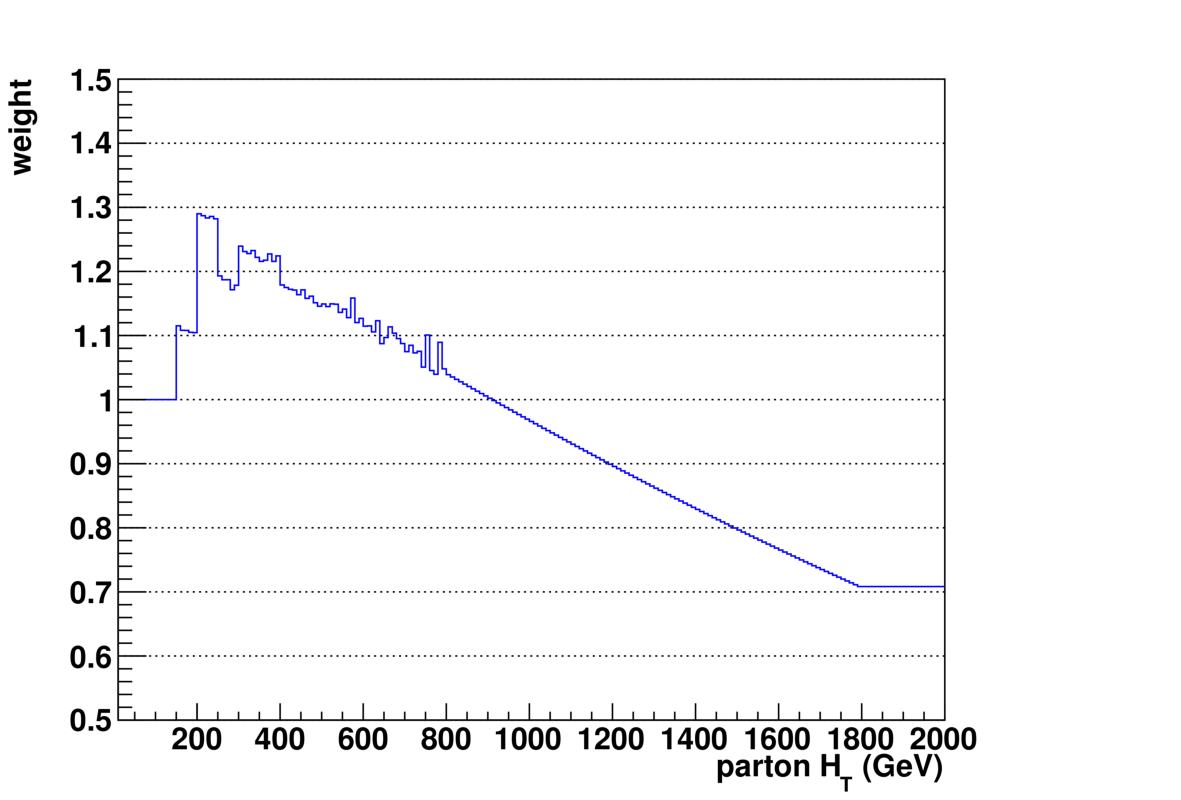
\includegraphics[width=0.6\textwidth,]{figures/samples/xs_wj_lv_mg_ht_incl_over_excl-7.pdf}
    } 
    \caption{Generator-level \partonht distributions and measured weights}
    \label{fig:xsec_study}
  \end{center}
\end{figure}

%The leading-order cross sections for each binned sample are corrected using
%a three-step process, described below.

%{\bf Step 1:} 
As a first step, we wish to reweigh the cross sections of the \partonht binned samples such that
their \partonht distributions match that of the inclusive sample's. Due to
the inclusive sample's limited statistics in the tails of \scalht distribution, 
we instead use the \nparton binned's \partonht distribution which is verified to agree well 
with the inclusive sample Figure~\ref{fig:xsec_study}~(a).  Additionally, to smooth statistical
fluctuations, both distributions are fitted using a double exponential of the form $exp(a+bx + cx^{1.05})$
for \scalht $> 500\gev$, Figure~\ref{fig:xsec_study} (b). The ratio of the distributions,
shown in Figure~\ref{fig:xsec_study}(c), is applied as \partonht dependent event weight.

In the high-\scalht and high missing energy corner of kinematic phase space of this analysis 
(and other SUSY analyses) the overall normalization of MC samples does not 
agree well with data. Therefore a data sideband in \scalht is used
to determine sample-specific corrections that are appropriate for the
\scalht-\met phase space covered by this analysis. This correction is determined 
for the \wlnu and \ttbar samples by imposing requirements on the number of muons, 
jets, and b-tagged jets, to obtain samples rich in W + jets, and \ttbar events.
A sideband in \scalht is used to determine both the yields in data and
MC expectations. The sideband is defined by the bin $200 < \scalht
< 225\gev$ and uses the jet \pt thresholds ($73,73,37\gev$) to maintain 
comparable jet multiplicities, kinematics, and background admixtures as observed for the
higher \scalht bins. Trigger efficiency and b-tag scale factor corrections 
are determined and applied to the MC samples. The ratio of the selected process 
over the total SM background (purity) of the samples is $>80\%$ and
any contamination is taken into account. The correction is determined by 
taking the ratio of the data yield over the MC expectation in the sideband. 
Table~\ref{tab:xs} summarizes the selection and corrections for the different samples. 

%Finally, an important point to note is that the corrections to the
%cross sections, derived with data sidebands, are only relevant for
%data/MC comparison plots and the suite of closure tests defined in
%Sec.~\ref{sec:bkgd-syst}. The transfer factors used to predict the SM
%background counts, defined in Sec.~\ref{sec:backgrounds}, are {\it
%  not} sensitive to changes in the cross sections.
%
\begin{table}[!h]
  \caption{Corrections determined from a data sideband for the W + jets and \ttbar samples. 
  ``Corrected yield'' reflects the observed data yield minus the contamination as given by MC.}
  \label{tab:xs}
  \centering
  \footnotesize
  \begin{tabular}{ llcccc }
    \hline
    \hline
    Process                       & Selection                         & Purity & Corrected yield & MC expectation      & Correction Factor        \\
    \hline
    W + jets                      & \mj, \njetlow, $\nb = 0$          & 0.90   & 15682           & $18013.1 \pm 85.9$ & $0.87 \pm 0.01$ \\
    \ttbar                        & \mj, $\njet \geq 2$, $\nb \geq 2$ & 0.83   & 752           & $736.7 \pm 11.5$ & $1.02 \pm 0.05$ \\
    \hline
    \hline
  \end{tabular}
\end{table}
